\section{IntelliJ IDEA}
\author{Benjamin Besic}

IntelliJ IDEA ist eine der führenden Entwicklungsumgebungen für die Programmiersprache Java. Sie wurde vom Unternehmen Jetbrains im Jahre 2000 entwickelt.
\\* Außerdem bietet sie ebenfalls Entwicklungsmöglichkeiten für Kotlin, Groovy, Scala und auch Android.
 Sie ist immer auf dem neusten Entwicklungsstand, wird laufend mit Updates versorgt und unterstützt die derzeit gängigen Programmiertools
wie Docker, Kubernetes, Maven, Datenbank-Tools, Git, Jakarta EE und viele weitere.
Es gibt eine kostenpflichtige Ultimate Version und eine Community Version, die kostenfrei zur Verfügung gestellt wird.
\\* IntelliJ zeichnet auch die Anzahl an Erweiterungen mittels Plugins aus. Die Umgebung besitzt auch eine
sehr intuitive Intelligenz, die es dem Entwickler sehr einfach macht damit zu programmieren.
\cite{IntJ} \\*
Wir haben uns dafür entschieden, da wir damit viel Erfahrung hatten und die oben genannten Punkte
unterstützten unsere Entscheidung enorm.

\section{Android Studio}
\author{Bozidar Spasenovic}
Android Studio ist eine Entwicklungsumgebung für Android-Anwendungen.
\\* 
Neben dem leistungsstarken Code Editor werden noch mehr Funktionen, für die Produktivität, bereitgestellt. 
Android Studio funktioniert auf Windows, GNU/Linux, macOS und Chrome OS. Die erste Version kam, nach zwei Jahren Entwicklungsdauer, am 8. Dezember 2014 raus.
Weiters beinhaltet es ein Gradle-build-system, viele verschiedene Android Emulatoren, ein Vorschaufenster mit der Anwendung was bedeutet, dass es konstant aktualisiert wird. 
Es funktioniert mit den Programmiersprachen Java, Kotlin und C++. 

\section{Git}
\author{Benjamin Besic}
Git ist ein Versionskontrollsystem (oft abgekürzt durch VCS) für Entwickler. Es ist ein Open-Source System, das im Jahre 2005
von Linus Torvald entwickelt wurde. Laut einer Stack Overflow-Umfrage von Entwicklern nutzen über 87 \% der Entwickler Git.
\cite{GitKinsta}
\\* Zu aller erst muss man den Begriff Versionskontrolle erklären, um Git zu verstehen.
\subsection{Versionskontrolle}
Diese dient dazu, um den originalen Quellcode effizient mit mehreren Personen editieren bzw. entwickeln zu können. 
\\* Die Entwickler arbeiten mit Verzweigungen und Zusammenführungen. Jeder Entwickler kann Änderungen sicher durchführen, ohne seine Kollegen dabei 
zu behindern. Diese Änderungen können dann, sobald sie funktionsfähig sind, wieder in den Hauptquellcode eingebunden werden.
Alle Änderungen sind zurückzuverfolgen und bei Bedarf kann man sie dann wieder zurücksetzen.
\cite{GitKinsta} \\*

\subsection{Git Funktionsweise}
Jeder Entwickler hat seine eigene Version des Projekts (Working Directory), die er frei bearbeiten kann. Diese bekommt man durch einen Klon des Projekts (\hyperref[sec:Clone]{Clone}). \\* Diese Änderungen kann man aufteilen und 
in Paketen bereitstellen, nach dem man diese durch Commits trennt. Einen \hyperref[sec:Commit]{Commit} kann man benennen. \\*
Diese Commits kann man dann online veröffentlichen durch einen \hyperref[sec:Push]{Push}. Ein Push ist nur möglich, wenn man die aktuellste Version des Projekts
auf seinen Rechner gezogen hat (\hyperref[sec:Pull]{Pull}). 
Einem Push kann man einen bestimmten Zweig (\hyperref[sec:Branch]{Branch}) zuordnen. 
\begin{figure}[htp]
    \author{David Ignjatovic}
    \centering
    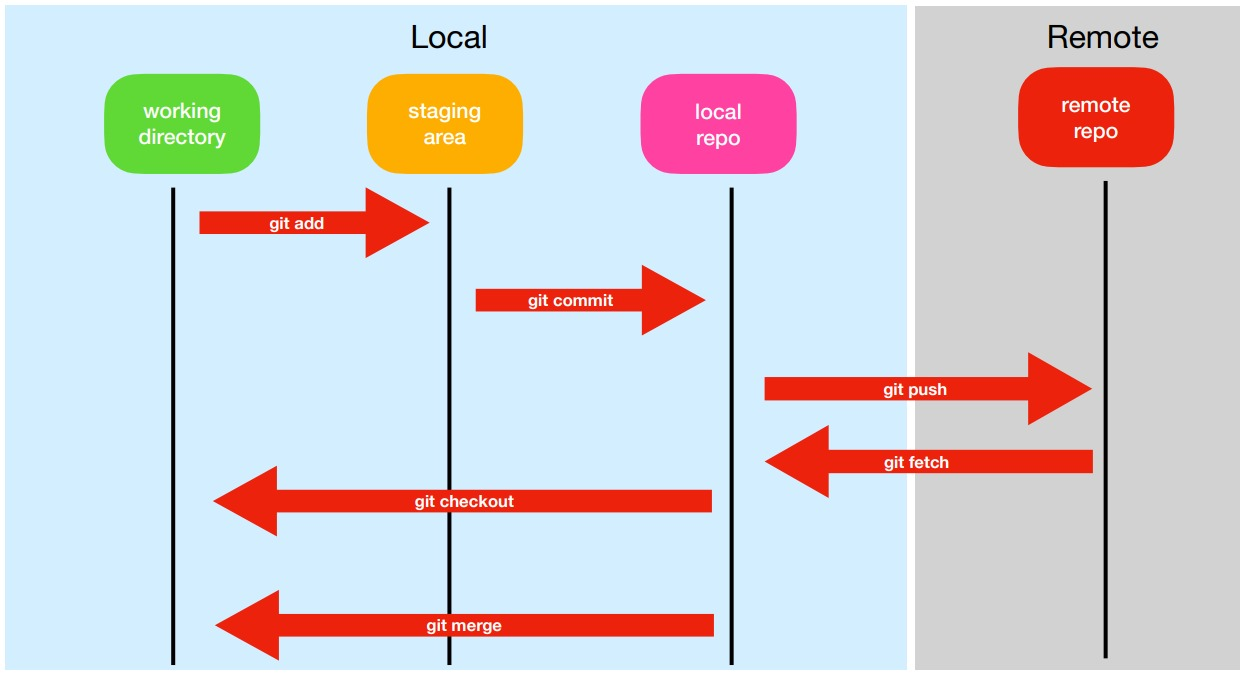
\includegraphics[scale=0.35]{pics/GitWorkflow.jpg}
    \caption{Darstellung des Git Workflows}
    \label{fig:impl:GitWorkflow}
\end{figure}
Diese Zweige dienen dazu, um das Projekt in verschiedene
unabhängige Teile zu trennen, falls man zum Beispiel an einer Demo Version weiterschreiben möchte. \\* Nach einem erfolgreichen Push sind die Änderungen
online auf dem Repository zu finden. Ein Repository ist der "Ordner", wo alle Dateien online gespeichert zu finden sind. 
\\* Ein Vorteil, den Git ebenfalls bietet ist das jeder Commit eine Version des Projekts ist, die man bis zum Zeitpunkt vom Commit herunterladen oder klonen kann.
Jedes Projekt kann privat oder öffentlich gemacht werden, sodass auch Personen, die keine Entwickler sind, darauf zugreifen können.
\cite{GitExpl} 



\subsection{Git Befehle}

\subsubsection{Clone}
\label{sec:Clone}
Es initialisiert ein Git Repository auf dem Rechner und ladet die zugehörigen Dateien runter.
Wenn man es nicht spezifisch angibt, klont es den Master Branch. Der Master Branch ist der Hauptzweig, eines jeden Git Projekts.
Innerhalb des erstellten Ordners können alle weiteren Git Befehle ausgeführt werden. \cite{GitCmnds}
\subsubsection{Commit}
\label{sec:Commit}
Ein Commit beschreibt Änderungen, die man im Projekt gemacht hat. Jeder Commit hat eine Bezeichnung, mit der der Entwickler die Änderungen,
die er gemacht hat beschreiben kann. Zu jedem Commit gehören auch die Dateien die dabei geändert bzw. hinzugefügt wurden.
\\* Es speichert den Zustand des gesamten Projekts bis zu dem Zeitpunkt und kann danach jederzeit abgerufen oder rückgängig gemacht werden.
Diese Änderungen bleiben aber zunächst nur lokal auf dem Rechner. \cite{GitCmnds}

\subsubsection{Push}
\label{sec:Push}

Ein Push dient dazu, um die lokalen Änderungen (Commits) zu veröffentlichen. Es kopiert den aktuellen, lokalen Stand und speichert diesen auf 
das vom Internet erreichbare Repository. \\* Einem Push kann ein Zweig (Branch) zugeordnet werden um die Änderungen zuzuordnen. 
Ansonsten wird der Master Branch genommen. \cite{GitCmnds}

\subsubsection{Pull}
\label{sec:Pull}
Der Pull Befehl kopiert die Inhalte vom öffentlichen Repository und fasst diese mit den lokalen Zustand auf dem 
rechner zusammen (merge). Es dient dazu die aktuelle Version des Projekts auf den Rechner herunterzuladen.
\\* Falls es Konflikte zwischen der derzeitigen und neusten Version gibt, werden die Änderungen zusammengeführt. \cite{GitCmnds}

\subsubsection{Branch}
\label{sec:Branch}
Die Branch Befehle dienen dazu um eine neue Abzweigung des Projekts (Branch) zu erstellen.
\\*
Branches erstellt man, wenn man an einer neuen Version des Projekts arbeitet und diese vom Hauptteil trennen will.
Meistens werden dadurch neue Funktionen programmiert, die später wieder in den Master Branch eingebunden werden.
\\* Der Vorteil daran ist, dass man an neuen Funktionalitäten experimentieren kann, ohne den Hauptentwicklungsstand zu 
beeinflussen. Branches können jederzeit gelöscht oder wieder ins Hauptprojekt integriert werden.
Es kann simultan am Master Branch und an Nebenzweigen gearbeitet werden durch trennen mit dem Push Befehl. \cite{GitExpl}

\begin{figure}[htp]
    \author{David Ignjatovic}
    \centering
    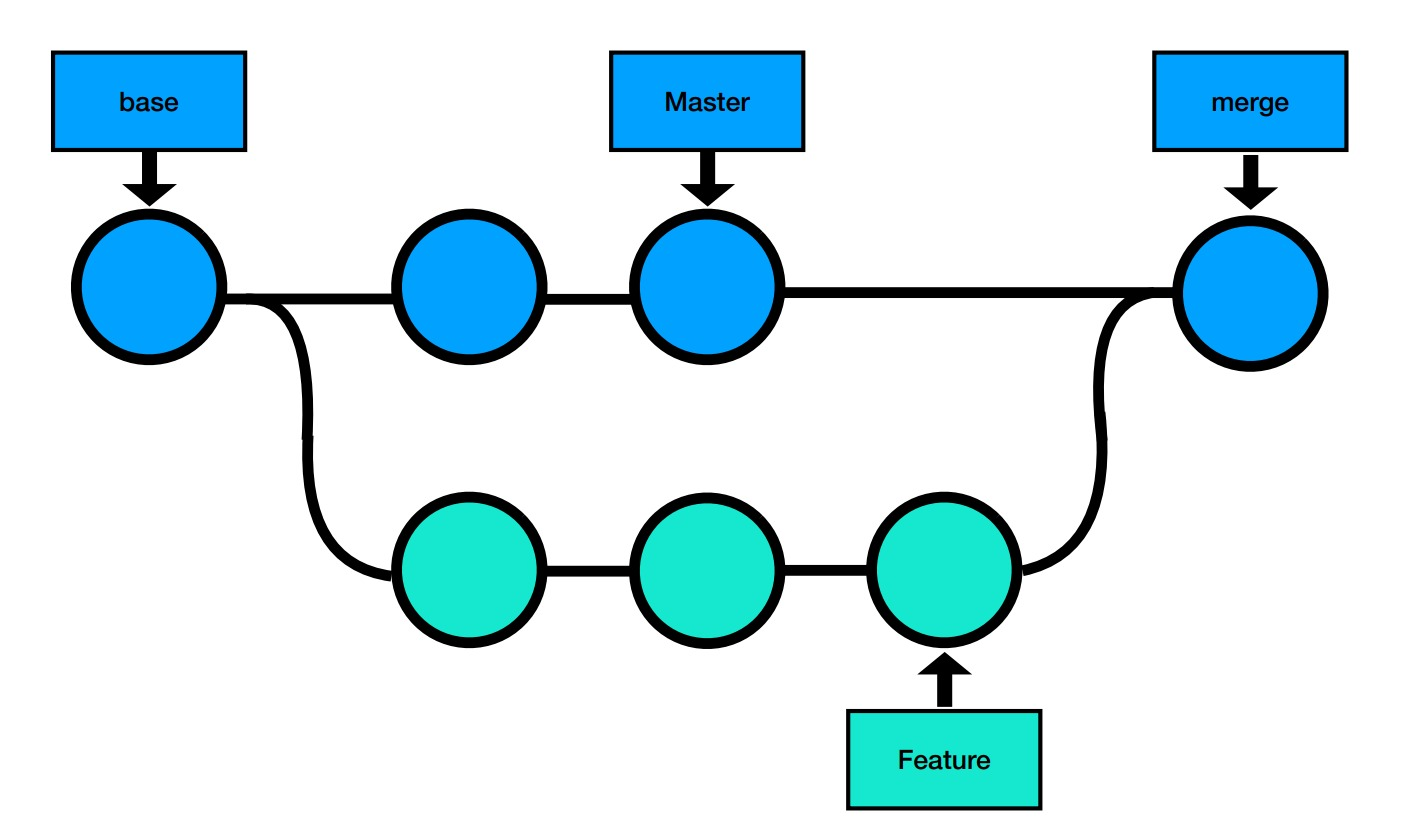
\includegraphics[scale=0.3]{pics/GitBranches.jpg}
    \caption{Darstellung von Branches in einem Repository}
    \label{fig:impl:GitBranches}
\end{figure}

\subsection{GitHub}
GitHub ist ein gewinnorientiertes Unternehmen, dass einen auf Cloud basierten Git Repository Hosting-Service anbietet.
Es wurde im Februar 2008 gestartet und von Chris Wanstrath, PJ Hyett, Scott Chacon und Tom Preston-Werner entwickelt.
Es ist das beliebteste Tool um Softwareprojekte zu verwalten und wird von über 73 Millionen Entwicklern und über 4 Millionen Organisationen
benutzt. Dazu ist es das größte und am meisten fortgeschrittene Entwicklungssystem, das es gibt. \cite{GitHub} \\*
Es vereinfacht die Nutzung von Git für Teams und auch Einzelpersonen. 
Jeder kann sich einen GitHub Account erstellen und direkt loslegen und seine Arbeiten auf Repositories veröffentlichen.
Es ist nicht nur zwingend für Code-basierte Projekte verwendbar sondern auch Websiten erstellen und das Schreiben von Büchern ist möglich.
\\*
Was GitHub ausmacht ist die Benutzerfreundlichkeit und die Integration von Git. Außerdem bietet Github viele andere Funktionen wie zum Beispiel ein Projekt Board an,
was es erleichtert innerhalb eines Teams, Probleme besser lösen zu können. \\*
Es gibt ebenfalls bezahlte Pläne, die es vor allem Organisationen und Unternehmen leichter macht Unternehmensprojekte zu verwalten durch zusätzliche Funktionen.
\cite{GitKinsta}



\section{Java}
\author{David Ignjatovic} 

Die relativ junge Programmiersprache Java, welche 1995 entwickelt wurde, weckte schon von Beginn an das Interesse der Programmiergemeinschaft auf. \cite{Java} \\*
James Gosling, welcher ursprünglich aus Kanada abstammt, entwickelte die objektorientierten, plattformunabhängigen Programmiersprache Java. \cite{JavaErfinder} \\*
Die Programmiersprache Java ist Teil der Java-Technologie. Sie besteht im Wesentlichen aus dem Java Development Kit (JDK) zum Erstellen von Java-Programmen und dem Java Runtime Environment (JRE) für deren Ausführung. 
Die Programmiersprache selbst sollte aber nicht gleichgesetzt werden mit der Java-Technologie. \cite{JavaSprache}

\subsection{Hello World}
\author{David Ignjatovic} 
\begin{lstlisting}[language=Java,caption=Java File HelloWorld,label=lst:impl:foo]
    public class HelloWorld {
        public static void main (String[] args){
                // Ausgabe Hello World!
                System.out.println("Hello World!");
        }
    }
    \end{lstlisting}

\subsection{Java Runtime Environment }
\author{David Ignjatovic} 

Java Runtime Environment (JRE) führt Software aus, die in der objektorientierten Programmiersprache Java geschrieben ist. 
Denn bei Java benötigt der Computer im Vergleich zur Programmiersprache C eine Laufzeitumgebung „Java Runtime Environment“ für das Betriebssystem, um Java-Programme ausführen zu können. \cite{JRE}

\subsection{Java Virtual Machine}
\author{David Ignjatovic} 

Java Virtual Machine (JVM) ist eine virtuelle Maschine, welche plattformunabhängige Anwendungen ermöglicht. Sommit lassen sich Systemweit Java-Programme ausführen.
Die Plattformunabhängigkeit wird in Java durch das Zusammenspiel zweier Programme gelöst: \\*
Der Compiler wandelt den Quelltext, also die .java-Dateien, in einen sogennanten Java-Bytecode. Der Interpreter (Virtual Machine) führt dann den Java-Bytecode aus. \cite{JVM}

\subsection{Java Byte-Code}
\author{David Ignjatovic} 

Bytecode in Java ist der Grund dafür, dass Java plattformunabhängig ist. Sobald ein Java-Programm kompiliert wird, wird der Bytecode generiert. 
Genauer gesagt ist ein Java-Bytecode der Maschinencode in Form einer .class-Datei.

\section{Java EE}
\author{David Ignjatovic} 

Die Enterprise Edition der Java Plattform (JEE), eine Spezifikation der Java-Plattform. 
Der wichtigste bestandteil von Java EE sind die Webanwendungen. Um solch eine Anwendung ausführen zu können, wird eine Applikationsserver verwendet, welcher 
in mehrere Systeme unterteilt wird, die auch Container gennant werden. Für eine Webanwendung reicht meistens reicht ein einzelner Web-Container aus. \\*

Die erste Version von Java EE, welche damals noch Java2EE genannt wurde, erschien im Jahr 1990. Im Jahr 2003 wurde der Name der Plattform auf Java EE geändert.
Die erste richtige Version von Java EE, welches wir bis heute noch kennen, erschien im Mai 2006 und trug die Versionsnummer 5. 2009 folgte die Version 6 und 2013 die Version 7.

Wie schon berreit erwähnt, wird zum ausführen einer Java EE Webanwendung ein Applikationsserver verwendet. Die am meisten verwendeten Applikationsserver sind so gennante 
Open-Source-Server wie zum Beispiel Apache Geronimo und GlassFish. 
Als Alternative zu einem vollständigen Applikationsserver können auch Programme verwendet werden, welche nur einen Web-Container implementieren.
Diese Web-Container werden oft auch als Servlet- oder JSP-Container bezeichnet und sind meistens dafür ausrecheichend. Der bekannteste Web-Container ist Apache Tomcat.

\cite{JavaEE}

\section{Quarkus}
\author{David Ignjatovic} 

Quarkus ist ein cloud-nativer Stack welcher von Red Hat entwickelt wurde. Es basiert auf den Jakarta EE- und MicroProfile-Standards. 
Eine Quarkus-Applikation hat gegenüber ein Konkurrenzprodukt eine deutlich kürzere Startzeit und einen erheblich geringeren Speicherbedarf, was ein großer vorteil ist für das Serverless Computing.  \cite{Quarkus} \\*

Quarkus wurde für entwickelt um de entwicklern die möglichkeit zu geben, applicationen für die moderne, cloud-native welt zu erstellen. 
Es ist ein Kubernetes-natives Java-Framework, das auf GraalVM und HotSpot angepasst wurde. Noch dazu wurde es aus erstklassigen Java-Bibliotheken und Standards erstellt. \\*   

Im März 2019 wurde Quarkus nach mehr als einem Jahr interner Entwicklung der Open-Source-Community vorgestellt

\subsection{Java EE vs. Quarkus}
\author{David Ignjatovic} 

Der größte Unterschied zwischen Java EE und Quarkus ist, dass man bei Quarkus keinen Application Server benötigt. 
Ein weiter Vorteil währe, dass bei Quarkus keine war-File erstellt wird, sondern eine jar-File, welche dem entsrpechend sehr klein ist. 
In diesem jar-File befinden sich auch noch die einzelnen Libaries, welche für die Webanwendung verwendet werden. \\*

Im gegensatzt zu Java EE wird eine war-File erstellt. Noch dazu befinden sich auf dem JEE-Application Server schon viele Libraries die schon vorinstalliert sind. 
Der größte Nachteil von Java EE ist, dass man auch für kleine Anwendung einen ganzen Application Server braucht. \\*

Im Großen und Ganzen kann man sagen, dass Quarkus hier dominanter ist, da es sehr praktisch und schnell ist. Noch dazu ist Quarkus relativ neu und kann sich im Laufe der Jahre noch umso mehr verbessern.



\subsection{JPA}
\author{David Ignjatovic} 

Java Persistence API (JPA) ist eine API welche für Datenbankzugriffe und für das objektrelationales Mapping verwendet wird. 
Objektrelationales Mapping (ORM) zeigt eine objektorientierte Sicht auf Tabellen und Beziehungen in relationalen Datenbank-Management-Systemen an.  \\*

Enterprise Applikationen führern üblicherweise viele Operationen auf Datenbanken durch.
Um aber eine Datenbankanbindung zu haben, müsste man sehr viel Code schreiben.
Durch die Hilfe von JPA (Java Persistance API) wird der aufwand reduziert, welcher benötigt wird, um mit der Datenbank zu komunizieren. \\* \cite{JPA}

JPA wurde von JSR 220 Expert Group entwickelt und im Mai 2006 erstmals veröffentlicht. 

\subsection{Hibernate}

Hibernate wird oft als Object Relational Mapping Tool bezeichnet. Es ist ein Framework zur Abildung von Objekten auf relationaler Datenbank für die Programmiersprache Java.
Hibernate implementiert die Java Persistence API (JPA)und bietet Funktionalitäten wie zum Beispiel  Datenbankabfragen mit der sogennanten Hibernate Query Language (HQL). \\*

Es wurde von JBoss im Jahr 2001 entwickelt und veröffentlicht. Sommit ist auch Hibernate in dem Boss Applikations-Server integriert .\cite{Hibernate}


\section{JBoss}

Red Hat JBoss Enterprise Application Platform (JBoss EAP) bietet Sicherheit und Performance. Der JBoss EAP ist eine Open-Source-Java EE-basierte Laufzeitplattform für Anwendungsserver.


\subsection{Panache}

Panache ist eine Quarkus-spezifische Bibliothek, welche die Entwicklung einer Hibernate-basierten Persistenzschicht vereinfacht. 
Panache ersetzt den größten Teil des Boilerplate-Codes mit einfachen methoden die man in die Quarkus Anwendung implementieren kann. 
Methoden wie create, update, and remove aber auch eigene Abfragen auf der Datenbank werden von Panache zur Verfügung gestellt. \\* \cite{Panache}

\section{Maven}


Apache Maven ist ein leistungsfähiges Werkzeug, welches immer weider vorkommende Prozeduren automatisiert und vereinfacht. 
Es wird oft als "Build Management System" bezeichnet und ist Teil vom "Software Configuration Management (SCM)".  \\* \cite{Maven}

Neben Maven gibt es auch noch ANT was eher kommandoorientiert arbeitet. Maven ist eher strategisch orientiert, realisiert mehr Abstraktionen, wird deklarativer gesteuert, 
berücksichtigt Abhängigkeiten besser und ist besonders für aufwändigere Multimodulprojekte geeignet. \cite{Maven}


\section{Cypress}

\section{Keycloak}
\author{Benjamin Besic}
Keycloak ist eine Open-Source Software, die Single-Sign On mit Identity und Access Management für moderne Applikationen bereitstellt. Der erste Release war 2014 als Wildfly Community Projekt, seit 2018 aber steht es unter der Verwaltung von RedHat. \cite{KeycloakWiki}  \\* 
Es hat mehrere Distributionen und ist mit einer Vielzahl von Frameworks und Tools kompatibel bzw. integriert wie z.B.: Quarkus, Angular, Vue.js, Spring, usw. \cite{KeyCloakDZone}

\subsection{Distributionen}
\subsubsection{Server}
Die Standalone Applikation ist downloadbar als .zip auf der Keycloak Seite. Es gibt zwei Versionen vom Server, zu einem die Wildy Application Server Version und auch eine Version, die über Quarkus läuft.
\subsubsection{Docker Image}
Genau so wie beim Server gibt es auch hier zwei verschiedene, offizielle Docker-Images, eins, dass auf dem Wildfly Server basiert und eins, dass auf Quarkus basiert.
\subsubsection{Operator}
Dies ist eine Distribution für Kubernetes und OpenShift, basierend auf der Operator SDK. \cite{KeyCloakDZone}
\subsection{IAM (Identity Access Management)}
\label{sec:IAM}
Eine der Hauptfunktionen von Keycloak ist das IAM. \\*
IAM oder auch IdM (Identity Management) ist ein Framework, das zum Authentifizieren von Benutzern und deren Rechten genutzt wird. \\*
Es prüft ob der Benutzer Zugang zu bestimmten Bereichen, Dateien und anderen Ressourcen hat, auf die er zugreifen will. Es prüft auch wer diese Rechte verändern darf.
IAM-Systeme stellen auch nützliche Admin-Tools zur Verfügung, um z.B. Nutzerrechte zu ändern oder die Aktivität von Benutzern zu verfolgen. \cite{KeycloakMakeIT} \\*
IAM hat vier Hauptfunktionen:
\begin{itemize}
    \item \textbf{Die Identitäts-Funktion: }Es umfasst die Erstellung von Identitäten (Benutzern), das Managen und Löschen von diesen.  
    \item \textbf{Die User Zugriff-Funktion (log-on): } Dies umfasst ein Interface, indem der Benutzer seine Zugriffsdaten eingeben (übermitteln) kann.
    \item \textbf{Die Service-Funktion: } Für Benutzer und deren Geräte stellt das System personalisierte, rollenabhängige, multimedia, online und on-demand Services zur Verfügung. \cite{KeycloakMakeIT}
\end{itemize}

\subsection{Single Sign-On (SSO)}
\label{sec:SSO}
SSO ist eine Variante der Zugangskontrolle, deren sich Keycloak bedient. \\*
Es ist für mehrere und zusammenhängende Softwaresysteme gedacht, wo der Benutzer nur einmal sein Passwort und Benutzernamen eingeben muss, um auf alle Systeme zugreifen zu können,
ohne sich dazwischen neu identifizieren zu müssen.\\* SSO ist typischerweise zu ermöglichen mit LDAP (Lightweight Directory Access Protocol). Bei IP-Netzwerken funktioniert das Ganze über Cookies, die gespeichert bleiben 
und die Seiten müssen eine gleiche, übergeordnete DNS Domain haben.\\* 
Authentifizierungsschemas, die dies unterstützen sind: OAuth, OpenID, OpenID Connect und Facebook Connect. Diese ermöglichen das Einloggen über mehrere verschiedene Websites mit den selben Anmeldedaten.\cite{KeycloakMakeIT}
\subsubsection{Vorteile von SSO}
\begin{itemize}
    \item Reduziert das Risiko beim Verwenden von Drittanbieter-Websites
    \item Reduziert die Passwortschwäche von den verschiedenen User und Passwort Kombinationen.
    \item Reduziert die Zeit, die man für das Eingeben der verschiedenen Identitäten braucht
    \item Reduziert IT-Helpdesk Anrufe wegen Passwörtern, daraus werden auch die IT-Kosten reduziert \cite{KeycloakMakeIT}
\end{itemize}

\subsection{OAuth 2.0}
Es ist möglich mit Keycloak den Standard OAuth 2.0 umzusetzen. \\*
OAuth 2.0 ist ein offener Standard, der im Oktober 2012 als Überarbeitung des Standards OAuth veröffentlicht wurde. \\*
Er behandelt ausschließlich den autorisierten Zugriff eines Benutzers auf eine Ressource. Wichtig zu beachten ist, dass er die Identität nicht überprüft. \\*
Ein Anwendungsfall von OAuth wäre einen Client zu verwenden, um Neuigkeiten auf einem Social-Media Profil zu veröffentlichen. Der Client holt die Autorisierung dazu aus der Social-Media Plattform. \cite{OAuthIonos} \cite{KeycloakCodeCentric}
\pagebreak

\subsubsection{Ablauf von OAuth 2.0}
\begin{figure}[htp]
    \centering
    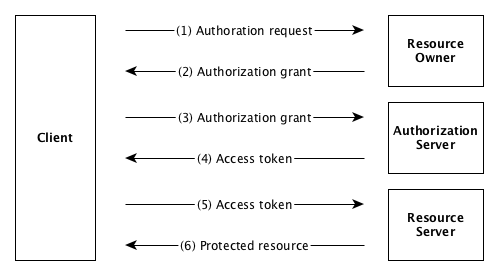
\includegraphics[scale=0.8]{pics/Ablauf_OAuth2.png}
    \caption{Ablauf des OAuth 2.0 Protokolls}
    \small \url{https://miro.medium.com/max/1400/1*1McvnvrW6wh37ECYpmTSxw.png} 
    \label{fig:impl:OAuth2Protocoll}
\end{figure}

Diese Grafik beschreibt den Weg, den der Client geht, um sich die Rechte auf die bestimmte Ressource (z.B. Veröffentlichung eines Beitrags) zu sichern. \\*
Wie man an der Grafik erkennen kann kommuniziert OAuth 2.0 nicht mit dem Benutzernamen und Passwort des Benutzers. 
Als Kommunikationsgrundlage dient ein Access-Token, dieser kann jeder Zeit ungültig gemacht werden, somit verliert der Client auch die Rechte auf die Ressource. \cite{KeycloakCodeCentric}

\subsection{OpenID Connect (OIDC)}
Mit Keycloak ist es ebenfalls möglich OIDC umzusetzen bzw. zu benutzen. \\*
OpenID Connect ist ein Authentifizierungs- und Autorisierungsprotokoll, dass im Februar 2014 von der OpenID Foundation veröffentlicht wurde.
Es erweitert die Funktionalität von OAuth 2.0 und benutzt dazu auch JWT (JSON Web Tokens). \\*
OpenId Connect soll die zentrale Stelle zur Verwaltung eines Benutzerprofils sein. Somit läuft auch jeder Authentifizierungsprozess über diesen ab.
Der Browser soll quasi die zentrale Komponente im Internet darstellen und jede Website benutzt die selbe OIDC Authentifizierung. Somit werden einem mehrere Benutzeraccounts gespart. \cite{KeycloakCodeCentric}
\pagebreak

\subsubsection{Ablauf von OIDC}
\begin{figure}[htp]
    \centering
    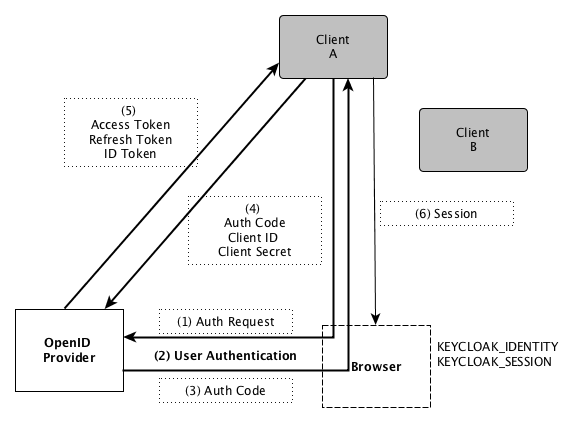
\includegraphics[scale=0.6]{pics/Ablauf_OIDC.png}
    \caption{Ablauf des OIDC Protokolls}
    \small \url{https://blog.codecentric.de/files/2016/08/openidconnect1.png} 
    \label{fig:impl:OIDCProtocoll}
\end{figure}

Der Browser leitet anfangs den Benutzer zum OpenID Provider hin, wo man sich beispielsweise mit Benutzername und Passwort authentifiziert.
Danach bekommt der Client einen Auth-Code, dieser wird dann zum Access, Identity und Refresh Token umgewandelt.
Der Client wird durch Keycloak verifiziert, indem er vorher bei Keycloak mit einem Secret und einer ID konfiguriert wurde. Dies dient dazu, damit kein willkürlicher Client diese Information erhalten kann.
In dem ganzen Prozess muss aber sichergestellt sein, dass jede Komponente das Secret sicher bewahren kann.
Zu allerletzt setzt der Browser dann die Session vom Benutzer und diese bleibt auch. \cite{KeycloakCodeCentric}

\subsubsection{Unterschied zu OAuth 2.0}
Der initiale Ablauf ähnelt dem von OAuth 2.0, doch der große Unterschied liegt in den Tokens.
Bei OIDC wird ein JWT (Json Web Token) übergeben. Dieser enthält Informationen zur Identität und zu den Attributen des Benutzers.
Diese können dann von der Applikation benutzt werden. \cite{KeycloakCodeCentric}


\subsection{Features}
\subsubsection{Multiple Protocols Support}
Gerade unterstützt Keycloak drei verschiedene Authentifizierungsprotokolle: OpenID Connect, OAuth 2.0 und SAML 2.0 \cite{KeyCloakDZone}
\subsubsection{SSO (Single Sign-On)}
\hyperref[sec:SSO]{Siehe hier}
\subsubsection{Admin Konsole}
Keycloak stellt eine web-basiertes Interface zur Verfügung, wo der Admin seine Konfigurationen intuitiv vornehmen kann. \cite{KeyCloakDZone}
\subsubsection{User Identity und Accesses}
\hyperref[sec:IAM]{Siehe hier}
\subsubsection{External Identity Source Sync}
Wenn man ein eigene User-Datenbank  hat, kann man diese mit Keycloak verbinden und synchronisieren. Standardmäßig unterstützt es LDAP und Active Directory, aber diese
kann man durch selbstgeschriebene Extensions erweitern. Diese kann man mit der Keycloak User-Storage API machen. Es garantiert aber nicht, dass Keycloak alle Funktionen aufweist,
die auch die Datenbank hat. \cite{KeyCloakDZone}
\subsubsection{Identity Brokering}
Keycloak kann auch als Proxy zwischen den Usern und einem oder mehreren externen Identity Provider fungieren. Diese können im Admin Panel editiert werden. \cite{KeyCloakDZone}
\subsubsection{Social Identity Providers}
Zusätzlich erlaubt Keycloak die Benutzung von Social Identity Providern. Es hat eine eingebaute Unterstützung für Google, Twitter, Facebook, Stack Overflow, diese müssen aber 
im Admin Panel manuell konfiguriert werden. Die volle Liste der kompatiblen Social Identity Provider kann in der Keycloak Dokumentation gefunden werden. \cite{KeyCloakDZone}
\subsubsection{Anpassung von Seiten}
Keycloak erlaubt eine Anpassung aller Seiten, die dem User angezeigt werden (z.B. Login-Page). Diese sind im .ftl Format, somit kann man klassisches HTML und CSS zum editieren verwenden.
Auch Javascript steht zur Verfügung, damit ist der Anpassungsspielraum unendlich. \cite{KeyCloakDZone}
\pagebreak

\subsection{Funktionsweise}
\begin{figure}[htp]
    \centering
    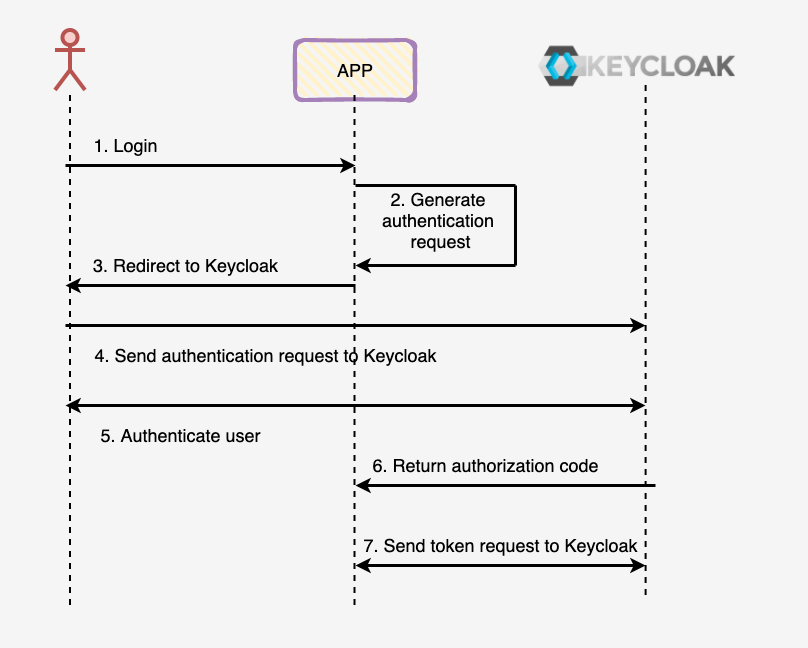
\includegraphics[scale=0.55]{pics/Keycloak-Funktionsweise2.png}
    \caption{Keycloak Funktionsweise}
    \small \url{https://miro.medium.com/max/1400/1*1McvnvrW6wh37ECYpmTSxw.png}
    \label{fig:impl:KeycloakFunc}
\end{figure}

Keycloak speichert sich einen Public Link der Applikation. Wenn dieser Link von einem User geöffnet wird, leitet Keycloak diesen zu einer Keycloak Authentication Page weiter.
Nachdem erfolgreichen Einloggen leitet Keycloak den User dann zu dem eigentlich gewünschtem Link weiter und gibt einen Token mit Zeitstempel mit.
Die Applikation kann dann den Token verwenden um den User und seine Rechte zu identifizieren. \cite{KeycloakMakeIT} \\*
\textbf{Bei der Funktionsweise sind wichtige Begriffe von Nöten:}

\subsubsection{Realm}
Ein Realm kann man sich als Mieter vorstellen, der einen Bereich zur Verfügung stellt. Dieser sogenannte Realm ist vollkommen isoliert (im Sinne von Usern, Konfigurationen, Rollen, etc.)
von anderen Realms. \\* Aus diesem Grund kann man einen internen Realm für z.B. Mitarbeiter machen und einen externen für z.B. Kunden. Somit sind die beiden von einander getrennt. \cite{KeyCloakCodex}

\subsubsection{Client}
Clients sind die Anwendungen, die eine Authentifizierung von Keycloak fordern, also z.B. eine Webapp. Diese können aber auch mobile oder native Applikationen sein.
Sie können jeder Servicetyp sein wie REST API's, gRPC oder WebSockets, die nur eine simple Authentifizierung und Rollenvergabe mittels Access Tokens benötigen. \cite{KeyCloakCodex}

\subsubsection{Rollen}
Eine Rolle repräsentiert eine Rolle in der Organisation bzw. in der Applikation. Ein User kann z.B. eine Admin-Rolle bekommen und somit alles an der Applikation konfigurieren.
Wenn man dies nicht will kann man Rollen und deren Spielraum eingrenzen, sodass die Applikation nicht willkürlich verändert wird. \\*
Keycloak unterstützt ebenfalls zusammengesetzte Rollen. Diese Funktion sollte man aber vorsichtig behandeln, da diese die Komplexität der Applikation erhöht und diese somit schwerer zu pflegen ist. \cite{KeyCloakCodex}

\subsubsection{User}
Der User ist der eigentliche Benutzer der Applikation. Dieser kann dementsprechend zu einem Realm gehören und seine eigenen Rechte haben.
Dieser identifiziert sich durch den Client und seine Rollen im Realm werden der Applikation mitgegeben.


\section{Oracle Datenbank}
\section{Vue.js}
\author{Benjamin Besic}
Vue.js ist ein JavaScript-Webframework, das zum Erstellen von Single-Page-Webanwendungen dient. 
Es wurde von einem kleinen Team im Jahre 2014 entwickelt mit dem ursprünglichem Autor Evan You.\\* Vue ist relativ neu und die große Stärke
von Vue ist die einfache Lernkurve, die Vielseitigkeit und die Leichtgewichtigkeit. Man benötigt Kenntnisse in JavaScript, HTML, CSS und schon kann man loslegen
mit deren ausführlich dokumentierten Guide\cite{VueGuide}. \cite{VueWissen} \cite{VueWiki}\\*

\subsection{Vue Funktionsweise}

\subsubsection{Model-View-Viewmodel (MVVM) Pattern }
Vue.js benutzt das MVVM Pattern. Das Pattern trennt die Darstellung von der Logik der Benutzer-UI's.
Dazu ist ein Datenbindungsmechanismus vorausgesetzt. Dadurch können sich Entwickler und Interfacedesigner trennen und ihre Aufgaben im Projekt 
aufteilen. \\*
Dieses Pattern wurde 2005 von John Gossman veröffentlicht. \cite{MVVM}

\begin{figure}[htp]
    \centering
    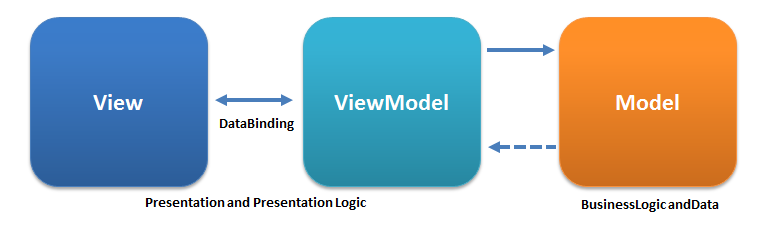
\includegraphics[scale=0.7]{pics/MVVMPattern.png}
    \caption{Darstellung von Branches in einem Repository}
        \small \url{https://upload.wikimedia.org/wikipedia/commons/8/87/MVVMPattern.png}
    \label{fig:impl:MVVM}
\end{figure}

\begin{itemize}
    \item \textbf{View:} Enthält alle Elemente die durch die Benutzeroberfläche angezeigt werden. Es bindet sich an das ViewModel, welches die Eigenschaften der View bestimmt.
    \item \textbf{ViewModel:} Es enthält die Logik des UI's. Es tauscht sich mit dem Model aus und benützt seine Methoden und Dienste. Gleichzeitig
          gibt es der View Eigenschaften, die dem Model entsprechen. Es bindet Daten mit der View und sich selbst (DataBinding).
    \item \textbf{Model:} Diese Schicht enthält alle Daten die der Benutzer manipuliert oder aufruft. Es enthält die gesamte Geschäftslogik.\cite{MVVM}
\end{itemize}

\clearpage

\subsubsection{Vue Instance}

Jede Vue Applikation beginnt mit der Erstellung einer Vue Instanz.

\begin{lstlisting}[language=JavaScript,caption=Vue Instanz,label=lst:impl:foo]
    var vm = new Vue({
        // options
    }) 
\end{lstlisting}

Die Variable vm steht für ViewModel, was unsere Vue Instanz darstellt. Man kann jeder Instanz Optionen zuweisen, um sie zu konfigurieren.
Diese Instanz wird auch als Root Instanz bezeichnet und bildet den Stamm eines Baumes mit Komponenten. 

\begin{figure}[htp]
    \centering
    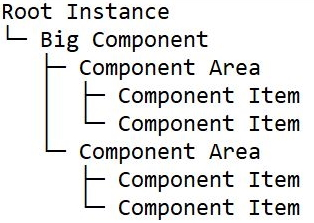
\includegraphics[scale=1]{pics/RootComponentTree.JPG}
    \caption{Der Stammbaum einer Root Instanz}
    \label{fig:impl:RootComponentTree}
\end{figure}
Zu einer Instanz gehört auch der data-Bereich. Dieser beherbergt alle Properties einer
Instanz und diese Properties reagieren auf Veränderungen im Code. Noch dazu kann jede Instanz Methoden haben. \\*
Jede Instanz hat auch seine Lifecycle Hooks, dies sind Methoden, die zu bestimmten Zeitpunkten einer Instanz ausgeführt werden. \cite{VueGuideInstance}
Diese sind:
\begin{itemize}
    \item \textbf{created}
    \item \textbf{mounted}          
    \item \textbf{updated} 
    \item \textbf{destroyed} 
\end{itemize}
\clearpage

\subsubsection{Lifecycle Diagram}
Das Diagramm hier stellt den Ablauf einer Erstellung einer neuen Vue Instanz dar.

\begin{figure}[htp]
    \centering
    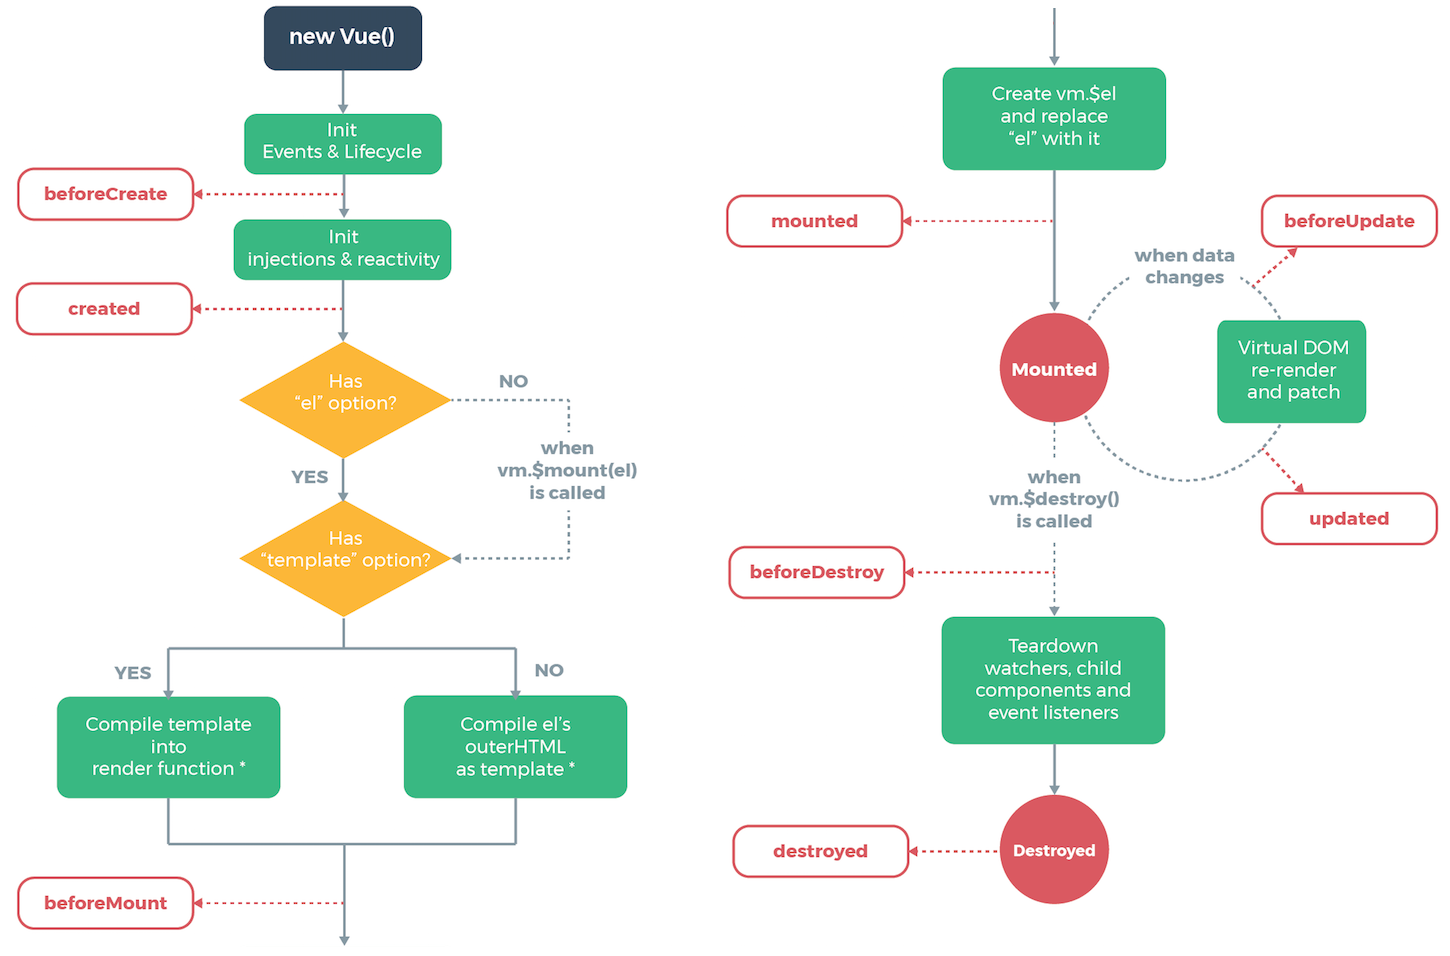
\includegraphics[scale=0.3]{pics/VueInstanceLifeCycle.png}
    \caption{Diagramm des Ablaufs einer Vue Instanz}
        \small \url{https://www.oreilly.com/library/view/full-stack-vuejs-2/9781788299589/assets/9f308e86-bbbe-489c-9f93-06abe2675081.png}
    \label{fig:impl:VueInstanceLifeCycle}
\end{figure}


\subsubsection{Vue Components}
Komponenten sind wiederverwendbare Vue Instanzen mit einem eigenen Namen. Diese Komponenten können mittels HTML-Tags in anderen Komponenten verwendet werden.
Eine Vue.js Seite ist meistens in mehrere Komponenten aufgeteilt, um größere Bereiche auf der Seite zu trennen und übersichtlicher zu gestalten. Diese können miteinander 
kommunizieren und Daten austauschen, um z.B. Daten, die ständig verändert werden ordentlich darzustellen.\cite{VueGuideComponents} \\*
\begin{figure}[htp]
    \centering
    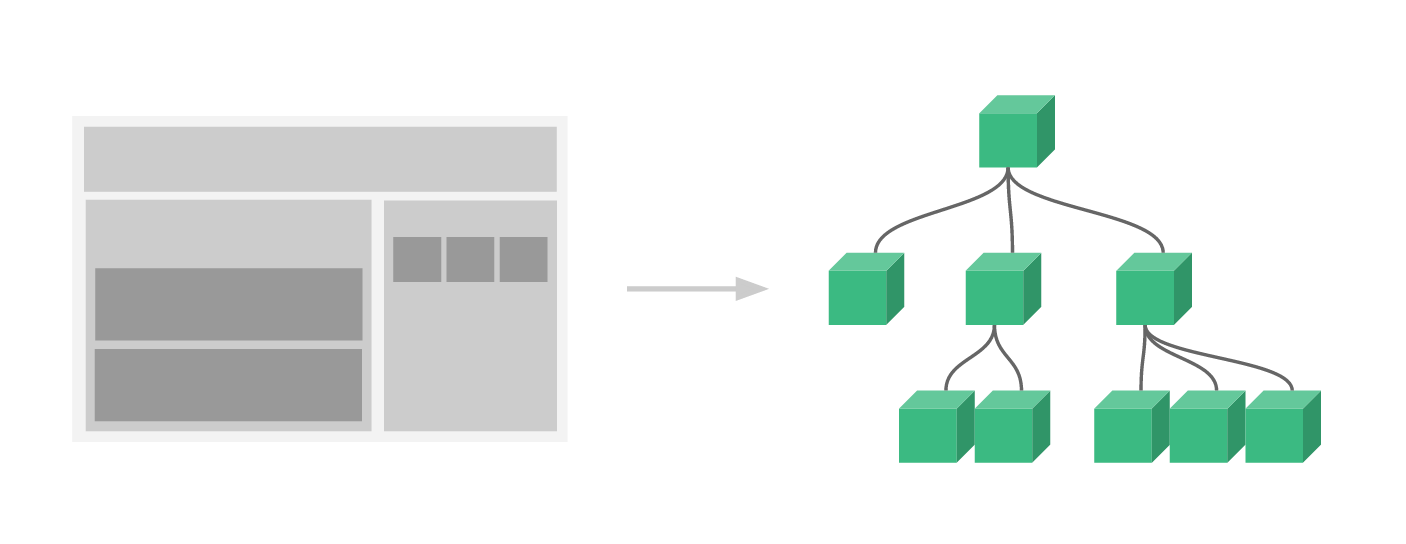
\includegraphics[scale=0.3]{pics/NestedComponentsTree.png}
    \caption{Darstellung von vernetzten Komponenten innerhalb einer Webpage}
        \small \url{https://vuejs.org/images/components.png?_sw-precache=b5c08269dfc26ae6d7db3801e9efd296}
    \label{fig:impl:NestedComponentsTree}
\end{figure}
Die folgende Grafik veranschaulicht den Component Tree, der zeigt wie die Single-Page Anwendung umgesetzt ist. 
Die grünen Boxen zeigen die miteinander vernetzten Komponenten, jeder Komponent kann mehrere Unterkomponenten haben, je nach Einteilung der Webseite.
\subsection{Angular vs. Vue}
\subsubsection{Marktstatistik}
\textbf{Angular:}
\begin{itemize}
    \item Angular wird eher für Seiten benutzt mit hohen Aufrufzahlen
    \item Nachdem was bekannt ist benutzen unter 0.4\% aller Webseiten Angular    
    \item Angular wird von 16.1\% Entwicklern weltweit verwendet \cite{AngVsVueSIM}
\end{itemize}

\textbf{Vue:}
\begin{itemize}
    \item Es gibt mehr als 1.523.449 Millionen Webseiten, die Vue benutzen
    \item Der Marktanteil von Vue beträgt nicht mehr als 0.5\% \cite{AngVsVueSIM}       
\end{itemize}
\subsubsection{Vor- und Nachteile}
Von der Lernkurve her ist Vue deutlich im Vorteil, da es einfacher zu verstehen ist als Angular. Angular benötigt viel Einarbeitungszeit, bis man die Funktionsweise
verstanden hat. Angular ist eher für umfangreiche Projekte gedacht, währenddessen Vue auf geringe Größe und hohe Performance abzielt. \\*
In Angular sind die Logik und das Aussehen strikt getrennt, währenddessen in Vue alles in einem File zu finden ist und mehr an HTML erinnert durch die Scripts, die man schreibt.
Ein Vorteil von Angular ist die Implementierung von Typescript, was eine Weiterentwicklung von JavaScript ist, die versucht die Macken von JavaScript zu verbessern.\\* 
Was noch zu erwägen ist ist, dass Angular weiter verbreitet ist als Vue und es oft Features oder Plugins gibt, die in Angular selbstverständlich sind, aber in Vue nicht aufzufinden sind.
Dies sollte sich aber im Laufe der Zeit verbessern. \\*  Generell kann man sagen, dass das Programmieren mit Angular eher and die Programmierung mit Java erinnert mit den Objekten, Abhängigkeiten,
Konstruktoren, usw. Während Vue an das Programmieren von Websites mittels HTML und JavaScript erinnert. \cite{AngVsVueHOST}
\subsubsection{Warum Vue?}
Unsere Entscheidung Vue zu nehmen ist einerseits von der Firma beeinflusst worden, da sie es vorgeschlagen haben und es bei ihnen das gängige Framework ist.\\*
Andere Faktoren waren noch, dass wir Angular in der Schule oft verwendet haben und wollten durch Vue eine andere Methode ausprobieren, um Webanwendungen zu erstellen.
Vue ist die bessere Wahl für den Umfang unserer Webanwendung gewesen und die bessere Performance in Vue ist wichtig, damit die Bestellungen reibungslos ablaufen können im Echtbetrieb.

\section{HTML}
\author{Benjamin Besic}
HTML genannt HyperText Markup Language, ist eine einheitliche, textbasierte, Auszeichnungssprache für Webdokumente. HTML definiert ganz allgemein gesehen die Struktur eines Dokuments. 
Am 13.März 1989 wurde am CERN in Genf das Konzept HTML von Tim Berners-Lee vorgeschlagen, um eine einheitliche Methode zu finden Dokumente öffentlich zu übermitteln. Seitdem ist HTML  einer Grundbausteine des World Wide Webs geworden. \\*
HTML basiert auf sogenannten Tags, die verschiedene Inhalte auf der Website definieren sollten. Diese basieren auf einer bestimmten Syntax, um das Schreiben zu vereinheitlichen. \\*
Es ist im Grunde eigentlich keine Programmiersprache, sondern eine statische Sprache, die zur Definierung benutzt wird. 
Das HTML Gerüst wird von einem Browser eingelesen und dieser generiert dann auf der Basis des HTML Files eine Website. \cite{HTMLTut} \cite{HTMLSeoKueche}

\begin{lstlisting}[language=HTML,caption=HTML File Grundgerüst,label=lst:impl:foo]
<!DOCTYPE html>
<html>
    <head>
        <title> Titel der Webseite </title>
    </head>
    <body>
        <h1> Ueberschrift </h1>
    </body>
</html>
\end{lstlisting}

Wie man im Beispiel sieht gibt bei Tags ein Beginn und ein Ende und der Inhalt dazwischen wird dargestellt.
Es gibt auch Tags ohne Beginn und Ende, sogenannte inhaltslose Tags.
Doch HTML wird meist nie allein verwendet, erst in der Kombination mit CSS, Bootstrap und JavaScript kann man eine gute Website erstellen.

\section{CSS}
\author{Benjamin Besic}
CSS (Cascading Style Sheets) ist die Sprache, die benutzt wird eine HTML Seite visuell zu gestalten. CSS ist wie HTML keine Programmiersprache, sie wurde dafür entwickelt um das Aussehen von HTML Seiten einheitlich zu verändern.\\*
Eine CSS-Datei wird durch einen Tag mit dem zugehörigen HTML Dokument verbunden und dadurch werden die Änderungen angewendet. \cite{CSSMozilla}

\begin{figure}[htp]
    \centering
    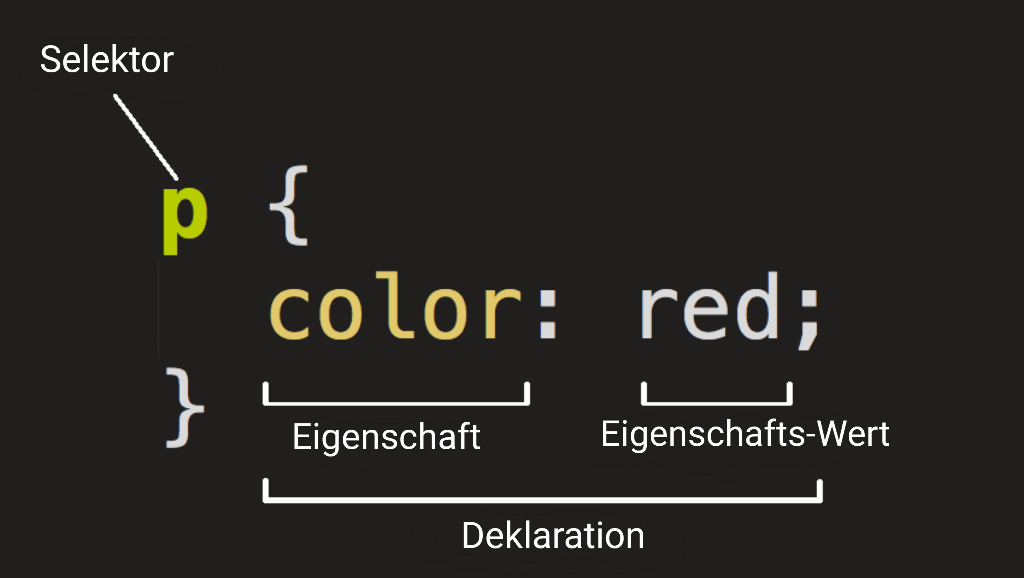
\includegraphics[scale=0.3]{pics/CSSRegel.png}
    \caption{Aufbau einer CSS-Regel}
        \small \url{https://media.prod.mdn.mozit.cloud/attachments/2017/09/27/15467/3889d04d90c10b27e863c6850d588c43/css-example.png}
    \label{fig:impl:CSSRule}
\end{figure}

Die Struktur von CSS-Dateien wird durch Regeln beschrieben. Jede Regel hat einen Selektor, der auf ein zugehöriges HTML Tag zugreift.
Innerhalb der Deklaration wird dann der Wert einer bestimmten Eigenschaft gesetzt (Mehrere Eigenschaften sind möglich).
Es gibt eine große Auswahl von Eigenschaften wie z.B.: Schriftfarbe, Textart, Positionierung, etc. \cite{CSSMozilla}

\section{JavaScript}
\author{Benjamin Besic}
JavaScript ist eine leichtgewichtige Skriptsprache, die 1995 vom Softwareunternehmen Netscape entwickelt geworden ist, um die Möglichkeiten von HTML und CSS zu erweitern.
Bekannt ist sie hauptsächlich als Sprache für Webseiten geworden, jedoch wird sie auch in vielen Umgebungen außerhalb des Browsers oft benutzt, wie z.B. Servern. 
\\* Sie unterstützt objektorientierte, imperative als auch deklarative Programmierung. JavaScript folgt dem Standard ECMAScript, welche alle Browser unterstützen. 
JavaScript dient dazu auf Webseiten Benutzerinteraktionen auszuwerten, Inhalte zu verändern, nachzuladen oder zu generieren. Sie bietet normalen HTML Webseiten eine Großzahl an Verbesserung, durch Hinzufügen von Programmierelementen. \\*
Jedoch sollte man JavaScript nicht mit der Programmiersprache Java verwechseln. Beide sind verschiedene Handelsmarken der Firma Oracle und ähneln einander höchstens mit der Syntax.
\cite{JSWiki} \cite{JSMozilla}
\section{JSON Web Token (JWT)}
\author{Benjamin Besic}
JSON Web Token ist ein nach RFC 7519 genormter Standard, um Daten sicher zwischen zwei Parteien auszutauschen. Es wird in der Form eines JSON-Objektes übertragen.
Die Information, die der Token enthält kann verifiziert werden, weil es eine digitale Unterschrift enthält. Der Token selbst kann entweder mit einem geheimen Schlüssel (HMAC-Algorithmus) oder einem private/public Schlüsselpaar (RSA oder ECDSA) verschlüsselt werden.\\*
Beliebte Anwendungsfälle des Tokens sind Authentifizierung und Datenaustausch. Der Token selbst enthält Informationen über den Absender und ob er die nötigen Zugriffsrechte hat.
\cite{JWTIO} \cite{JWTIONOS}
\subsection{Aufbau eines JWT}
Ein signierter JWT besteht aus 3 Teilen, getrennt durch einen Punkt. Jeder dieser Teile wird mit Base64 kodiert. \\*
Jeder JWT hat auch eine Gültigkeitsdauer, wenn diese abgelaufen ist, gilt ein Token als ungültig.
\clearpage
\begin{figure}[htp]
    \centering
    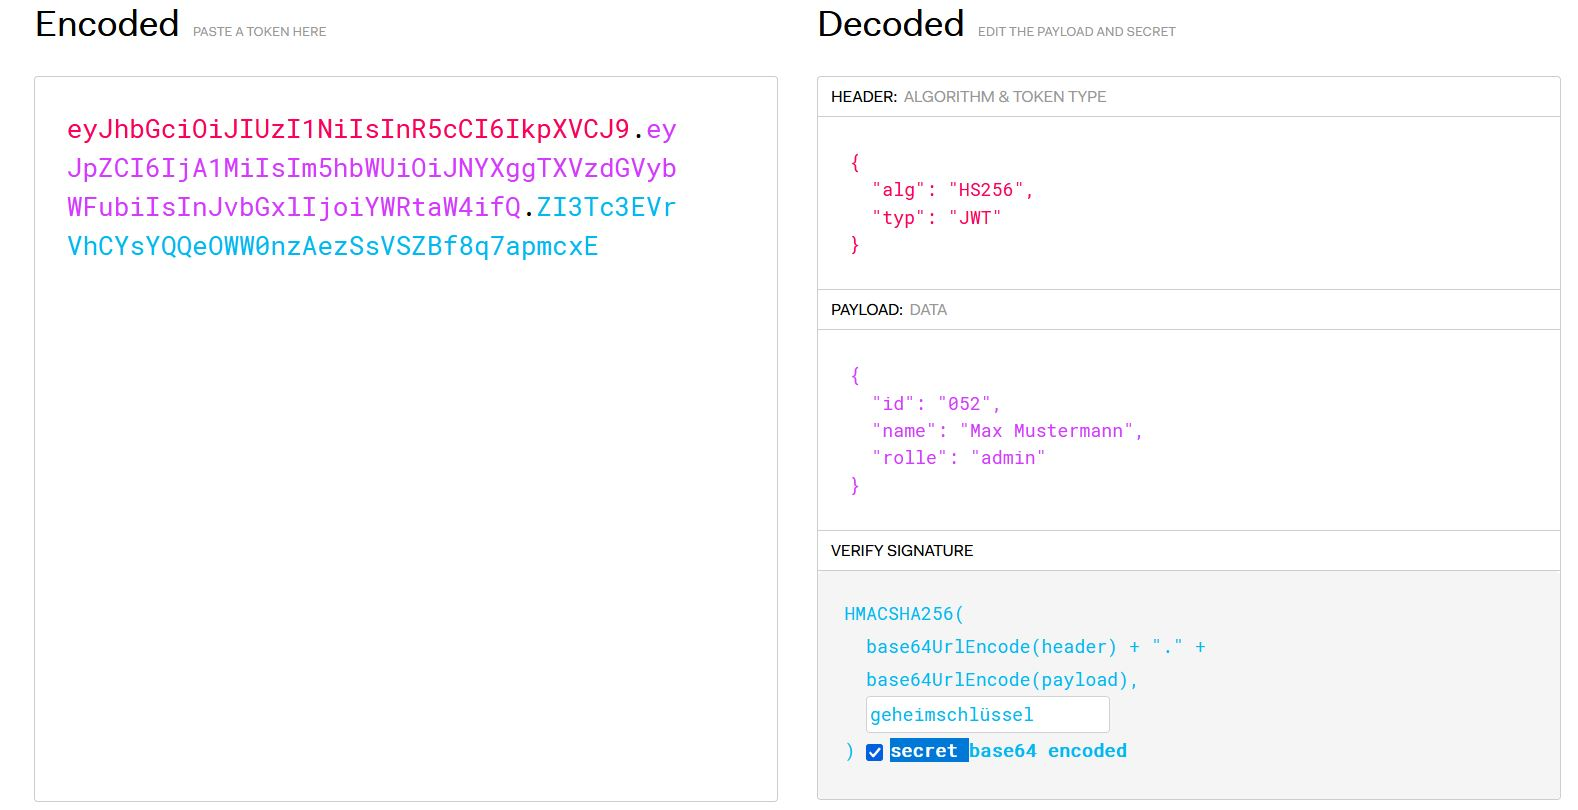
\includegraphics[scale=0.4]{pics/JWT.JPG}
    \caption{Aufbau eines JSON Web Tokens (Ausschnitt von jwt.io)}
        \small \url{https://jwt.io/}
    \label{fig:impl:JWT}
\end{figure}

\subsubsection{Header}
Der Header besteht meist aus zwei Teilen und liefert Informationen über den Typ des Tokens und den verwendeten Signatur- bzw. Verschlüsselungsalgorithmus.
\begin{itemize}
    \item Der "typ"-Wert beschreibt den IANA Medientypen des Tokens, oft wird "application/jwt" verwendet.
    \item Der "alg"-Wert gibt an welcher Algorithmus zum Signieren des Tokens verwendet wurde. Es ist möglich auch keine Verschlüsselung anzugeben, was jedoch nicht zu empfehlen ist. \cite{JWTIONOS}     
\end{itemize}
\subsubsection{Payload}
Der Payload ist der Teil des Tokens, der die tatsächlichen Daten bzw. Informationen enthält, die übermittelt werden sollen.
Sie werden als Key-/Value-Paare bereitgestellt, diese Werte werden bei JWT als Claims bezeichnet. \cite{JWTIONOS}  Davon gibt es drei verschiedene Arten:
\begin{itemize}
    \item \textbf{Registrierte Claims} sind standardisiert und im JWT Claim Register festgelegt. Es wird empfohlen diese zu verwenden.
    \item \textbf{Öffentliche Claims} sind nach belieben definierbar.
    \item \textbf{Private Claims} sind für Informationen gedacht, die speziell auf unsere Anwendung angepasst sind wie z.B. "Benutzer-ID". \cite{JWTIONOS} 
\end{itemize}

\subsubsection{Signature}
Diese wird durch Base64-Kodierung des Headers, des Payloads und der angegebenen Signaturmethode erzeugt. Der Aufbau ist definiert nach dem RFC 7515 Standard, auch genannt JWS (JSON Web Signature).
Damit die Signatur funktioniert, muss man einen geheimen Schlüssel verwenden, der nur dem Ursprung bekannt ist. \cite{JWTIONOS} 

\subsection{Sicherungsverfahren}
\subsubsection{Keine Sicherung}
Wenn die Daten keiner Verschlüsselung bedürfen, kann im Header "none" angegeben werden. In diesem Fall wird keine Signatur generiert, dadurch fällt auch der Signature-Teil weg. \\*
Ohne Sicherung lässt sich die Nachricht nach einer Base64-Entschlüsselung klar und deutlich lesen. Der Absender oder ob die Nachricht im Laufe verändert worden ist, ist nicht mehr verifizierbar.\cite{JWTIONOS} 
\subsubsection{Signatur (JWS)}
Im Normalfall reicht es nur zu prüfen, ob die Daten vom richtigen Absender kommen und ob Veränderungen geschehen sind. Da kommt die JWS (JSON Web Signature) zum Einsatz, die genau die vorher genannten Sachen überprüft.
\\* Bei diesem Verfahren lässt sich die Payload nach Base64-Entschlüsselung klar und deutlich lesen. \cite{JWTIONOS}
\subsubsection{Signatur (JWS) und Verschlüsselung (JWE)}
Es ist möglich zusätzlich zum JWS noch eine JWE (JSON Web Encryption) zu benützen. JWE verschlüsselt den Inhalt des Payloads, diese werden danach mit JWS signiert.
Um die Inhalte dann zu entschlüsseln wird noch ein Kennwort oder ein privater Schlüssel angegeben. \\*
Damit ist der Absender verifiziert, die Nachricht authentisch und der Payload ist nicht lesbar nach einer Base64-Entschlüsselung. \cite{JWTIONOS}
\section{Progressive Web App(PWA)}

\section{Google Charts}

\section{Jetpack Compose}
\author{Bozidar Spasenovic}
Jetpack Compose ist seit Juli 2021 in der ersten stabilen Version verfügbar. Es ist ein "Werkzeugkasten" zum Bauen von Android Applikationen.
Es vereinfacht und beschleunigt den Anwendungsentwicklungsprozess. Da man mit wenig Code schnell viele Ansichten erstellen kann, ist die Fehlerqoute dementsprechend niedrig.
Jetpack Compose basiert 100 Prozent auf Kotlin. Man kann zwischen drei Ansichten auswählen, die da Code, Split oder Design wären die das parallele arbeiten sehr vereinfacht. 
Das App wird aber nicht nach jeder änderung neu gebaut, was wiederum die Schnelligkeit des Arbeiten beeinflusst. Damit die Applikation eine schöne Oberfläche hat, bietet
Jetpack Compose mehrere Themes zu Verfügung. Noch dazu kann man diese dann auch selbst konfigurieren indem man Items hinzufügt oder löscht.
Jetbrains hat in Planung eine plattformübergreifendes Open-source Projekt zu starten, damit man Desktop Anwendungen genau so schnell und einfach erstellen kann. 

\section{Kotlin}
\author{Bozidar Spasenovic}
Kotlin ist eine universelle und statisch typisierte Open-Source-Programmiersprache, die ursprünglich für die Java Virtual Machine und Android entwickelt wurde.
Es konzentriert sich auf Interoperabilität, Sicherheit, Übersichtlichkeit und Werkzeugunterstützung. Als build-script wird Gradle verwendet.
\\*
2017 wurde sie zu einer offiziellen Sprache zur Entwicklung von Android-Applikationen. Deswegen wird Kotlin auch Programmiersprache der Zukunft betitelt wenn man sie mit Java vergleicht.
Lambdafunktionen werden deutlich reduziert und somit auch leichter in der Praxis als in Java. 
Da Kotlin sehr gut mit Java arbeiten kann, können beim Testen die Frameworks und Bibliotheken von Java sehr weiterhelfen.  
Ursprünglich hat man den Kotlin Code in Bytecode übersetzt und diesen dann in edr JVM laufen gelassen. 
Aber den Code kann man aber auch in Javascript umschreiben lassen und somit für Web Anwendungen verwenden.

\section{XML}
\author{Bozidar Spasenovic}
XML steht für eXtensible Markup Language und ist ein textformbasiertes Datenformat.
Das Wort eXtensible beschreibt die erweiterungsmöglichkeiten der Sprache.
Sie wurde im Jahre 1996 entwickelt und wurde zwe Jahre später zum W3C-Standart. 
Sie ist sehr leicht einsetzbar in verschiedene Anwendungen da sie keine Lizenz benötigt.
Viele Tools heutzutage erleichtern aber auch die bearbeitung von XML-Dateien.
Ein Vorteil ist, dass man die Daten im XML als Textformat abspeichert, was heisßt das XML auch plattformunabhängig ist.
Wie in HTML, gibt es auch hier sogenannte Tags, die aber selbst zu kofigurieren sind. 
Der große Vorteil von XML ist das es sehr leicht lesbar ist, sowohl von Mensch als auch von Machine.
Es wird in Android verwendet um das Layout jeder Aktivität des Android zu entwerfen und erleichtert die Datenübertragung zwischen Anwendungen.




\section{Docker}
\author{Bozidar Spasenovic}
Docker ist eine in GO programmierte Softwareplattform, die den Prozess des Erstellens, Ausführens und Verwaltens von Apps umfasst.
Dies geschieht durch Virtualisierung des Betriebssystems, auf dem es installiert ist und ausgeführt wird. 
\subsection{Docker Compose}


\section{OKHttp}
\author{Bozidar Spasenovic}
OkHttp ist ein HTTP-Client, der standardmäßig effizient ist. Dank der HTTP/2-Unterstützung ist es möglich alle Anfragen an einen Host zu schicken. 
 Response Caching hilft bei vermeidung von wiederholten Anfragen.
OkHttp hilft bei Verbindungsproblemen indem man alternative Adressen benutzt.
 OkHttp unterstürzt weiters noch TLS-Funktionen. Es kann so konfiguriert werden, dass es für eine breite Konnektivität zurückgreift.


\section{Gradle}
\author{Bozidar Spasenovic}
Gradle ist ein, in 2007 entwickeltes, Build-Management-Automatisierungs-Tool welches auf Java basiert.
Man kann es mit Apache Maven und Ant vergleichen.
Es hat die Flexibilität von Apache Ant und die simple Bediunungsmöglichkeit von Maven.
Der unterschied zu den  Maven-Projektdefinitionen ist, dass man Gradle-Scripts gleich ausführen kann.
 Gradle unterstütz neben Java noch die Programmiersprachen Groovy und Kotlin.
DAG wird verwendetr um die Tasks in richtiger Reihenfolge zu dirigieren.
Heutzutage hat Gradle eine eigene Maschiene für das verwalten der einzelnen Abhängigkeiten, aber es begann mit Apache Ivy.
\\* 
Seit Mitte 2013 ist Android hinzugekommen. Seitdem wurde das Tool weitgehend erweitert, um den Aufbau sogenannter „nativer“ Systeme zu unterstützen, welche nicht auf Java basieren.
Gradle wird von sehr großen Unternehmen verwendet wie zum Beispiel LinkedIn, Netflix, Adobe und vielen weiteren.


\section{Retrofit}
\author{Bozidar Spasenovic}
Über einen REST-basierten Webdienst wird es sehr einfach Daten hochzuladen oder auch abrufen. 
Retrofit ist ein REST-Client für Java und Android.
Es wird verwendet, um Requests zu Empfangen, Senden und Erstellen von HTTP-Anforderungen sowie Antworten.
Noch dazu wird die IP-Adressen ausgewechselt, wenn eine Verbindung zu einem Webdienstfehler besteht.